\documentclass[11pt]{article}

\usepackage[margin=1in]{geometry}
\usepackage[T1]{fontenc}
\usepackage[utf8]{inputenc}
\usepackage{lmodern}
\usepackage{microtype}
\usepackage{amsmath,amssymb}
\usepackage{booktabs}
\usepackage{tabularx}
\usepackage{array}
\usepackage{enumitem}
\usepackage{xcolor}
\usepackage{graphicx}
\usepackage{hyperref}
\usepackage{fancyhdr}
\usepackage{titlesec}
\usepackage{caption}

% Monochrome: a printed research paper, black on white.
\definecolor{accent}{HTML}{111111}
\definecolor{dark}{HTML}{111111}
\definecolor{muted}{HTML}{555555}
\definecolor{lightbg}{HTML}{FFFFFF}
\definecolor{line}{HTML}{111111}

\graphicspath{{../assets/}{./assets/}{../}}

\hypersetup{
    colorlinks=true,
    linkcolor=dark,
    citecolor=dark,
    urlcolor=dark,
    pdftitle={Neural Cup Pong: A Playable Action-Conditioned World Model},
    pdfauthor={Ryan Rahman}
}

\setlength{\headheight}{14pt}
\pagestyle{fancy}
\fancyhf{}
\lhead{Neural Cup Pong}
\rhead{Technical Report}
\cfoot{\thepage}
\renewcommand{\headrulewidth}{0.3pt}

\titleformat{\section}{\Large\bfseries\color{dark}}{\thesection}{0.75em}{}
\titleformat{\subsection}{\large\bfseries\color{dark}}{\thesubsection}{0.75em}{}
\titleformat{\subsubsection}{\normalsize\bfseries\color{dark}}{\thesubsubsection}{0.75em}{}

\setlist[itemize]{leftmargin=1.4em, itemsep=0.25em, topsep=0.25em}
\setlist[enumerate]{leftmargin=1.6em, itemsep=0.25em, topsep=0.25em}
\renewcommand{\arraystretch}{1.25}

\newcommand{\keybox}[1]{%
  \vspace{0.65em}
  \noindent\fcolorbox{line}{lightbg}{%
  \begin{minipage}{0.96\linewidth}
  \vspace{0.45em}
  #1
  \vspace{0.45em}
  \end{minipage}}
  \vspace{0.65em}
}

\newcommand{\vect}[1]{\mathbf{#1}}
\newcommand{\stt}{\vect{s}}
\newcommand{\act}{\vect{a}}
\newcommand{\code}[1]{\texttt{#1}}

\begin{document}

\begin{titlepage}
    \centering
    \vspace*{1.25cm}
    {\Large\color{accent}\textbf{Technical Report / Preprint}}\\[0.7cm]
    {\huge\bfseries Neural Cup Pong: A Playable Action-Conditioned World Model for 3D Cup Pong\\[0.35cm]}
    \vspace{0.45cm}
    {\large From a deterministic engine to a fully-generated, hand-controllable neural game, and the flight-precision wall in between}\par
    \vspace{1.2cm}
    \rule{0.82\linewidth}{0.5pt}\\[0.45cm]
    {\large Ryan Rahman}\\[0.15cm]
    {\normalsize University of Waterloo -- Mechatronics Engineering / Robotics Research}\par
    \vspace{0.45cm}
    {\normalsize \today}\par
    \vfill
    \keybox{\textbf{One-line summary.} A 409K-parameter GRU dynamics model plus a 262K-parameter state-grounded decoder together simulate and \emph{render} an entire arcade cup-pong game from controller input with no game engine and no graphics renderer in the loop; the ball's flight is the one place a small structured model cannot match ballistics, so a hybrid restores engine-parity sinking (6/6) while keeping control and rendering neural.}
    \vfill
    {\footnotesize A hobby project. All art, physics, and assets are original; nothing here reproduces a commercial title.\par}
\end{titlepage}

\tableofcontents
\newpage

\section{Abstract}

\emph{World models} learn to predict how an environment evolves under an agent's actions, and a growing line of work asks whether such models can be run \emph{as} the environment: a neural network the player controls directly, with no hand-written simulator or renderer \cite{worldmodels,diamond,gamengen,genie}. This report documents a small, self-contained instance of that idea: \textbf{Neural Cup Pong}, a playable action-conditioned world model for an original 3D cup-pong game (aim, charge power, throw a ballistic ball at a triangular rack of six cups).

The system is built in six stages: (1) a deterministic, seeded game engine with a fixed-camera 2.5D projection; (2) a scripted data-generation pipeline; (3) a \emph{structured} dynamics model, a gated recurrent network that predicts the next 21-dimensional game state from the current state and controller action, with a hard ``snap'' projection that keeps every prediction a legal game state; (4) engine-off inference, where the network alone advances the world; (5) a \emph{state-grounded latent renderer} that paints each $128\times96$ frame from state using rasterized geometry hints and FiLM conditioning; and (6) fully-generated play, where both the engine and the graphics renderer are switched off and the two networks produce the game end-to-end.

The learned model is near-perfect at the parts that matter for feel: it tracks aim and power with one-step errors of $0.0025$ and $0.0013$ (normalized), reproduces phase transitions at $99.4\%$ accuracy, and follows the player's controls with a $100\%$ directional-response rate. It is \emph{not} good at one specific thing: predicting exactly where a thrown ball lands. The GRU's predicted flight passes no closer than $\approx 8.4$ table-units to the target cup, versus $0.31$ for the engine, larger than a cup, so the fully-learned mode almost never sinks. We show this is a genuine capacity limit of a small structured model regressing a fast ballistic arc, not a training or class-imbalance artifact, and resolve it with a \emph{hybrid} world model: the network keeps driving aim, power, and phase, but the ball's arc is integrated with exact ballistics seeded from the network's own (accurate) aim/power at release. The hybrid sinks $6/6$ cups, matching the engine, while control stays neural and the decoder still renders every pixel.

\section{Introduction}

\subsection{Playable world models}

A world model is a learned simulator: given the current state (or observation) and an action, it predicts the next one. Classic formulations use them for imagination-based planning and reinforcement learning \cite{worldmodels,dreamerv3}. A more recent and more visceral use is to let a human drive the world model directly, turning it into a neural video game: GameNGen reproduces DOOM with a diffusion model \cite{gamengen}, Genie learns controllable environments from video \cite{genie}, and DIAMOND trains agents inside a diffusion world model of Atari \cite{diamond}. These systems are impressive but heavy. This project asks the opposite question: \emph{how small can a genuinely playable world model be, and what breaks first as you shrink it?}

Cup pong is a deliberate choice. It is simple enough that a deterministic engine fits in a few hundred lines, yet it contains the three ingredients that make world modeling interesting: (i) \textbf{continuous control} (aim and power the player trims in real time), (ii) \textbf{a ballistic event} (a thrown ball whose landing is a sensitive function of the launch), and (iii) \textbf{discrete, irreversible state changes} (a cup is present or sunk; the rack only empties). The last two turn out to pull in opposite directions, and the tension between them is the story of this report.

\subsection{Structured vs.\ pixel dynamics}

Rather than learn dynamics directly in pixel space, we separate concerns. A \emph{structured} dynamics model predicts a compact, interpretable game state (ball position, cup bitmask, phase, \ldots); a separate \emph{neural renderer} turns state into pixels. This mirrors the ``structured latent first'' discipline used to make world models controllable and debuggable before committing to pixels, and it lets us measure exactly which faculty (dynamics or rendering) is responsible for any failure. It also means the two networks can be tiny: $409$K and $262$K parameters respectively.

\subsection{Contributions}

\begin{enumerate}
    \item A complete, six-stage recipe for a playable action-conditioned world model of an original arcade game, small enough to train on a single consumer GPU and to run at interactive rates on CPU.
    \item A \emph{snap} projection operator that guarantees every learned state transition is legal (valid phase automaton, monotone cups, derived score, parked ball outside flight), used identically in training feedback and at inference.
    \item A \emph{state-grounded latent renderer} (SGLR) that reaches $L_1 = 0.0077$ reconstruction on held-out frames by feeding the decoder rasterized geometry hints plus a static court backdrop, rather than asking a conv net to invent the scene from a state vector.
    \item A clean diagnosis of the \emph{flight-precision wall}: a $\sim$409K structured model tracks control to $\approx 0.002$ but cannot localize a ballistic landing to within a cup radius ($8.4$u error), and no amount of loss re-weighting, event oversampling, or rule-based sink resolution fixes it because the predicted ball never reaches the cup.
    \item A \emph{hybrid} world model that restores engine-parity sinking ($6/6$) by integrating the ball's arc with exact ballistics seeded from the network's own aim/power, while leaving control and rendering fully neural: an honest, playable compromise and a concrete data point on what a small model should and should not be asked to learn.
\end{enumerate}

\section{The Game and the Deterministic Engine}

\subsection{Rules and camera}

The player faces a table (Figure~\ref{fig:phases}). Table-space uses $x$ across ($[0,60]$), $y$ in depth toward the cups ($[0,100]$), and $z$ up. Six cups sit in a triangular rack (rows of $3$, $2$, $1$) at $y\in\{74,82,90\}$. The player trims a lateral aim $\code{aim\_x}\in[-1,1]$ and a launch power $\code{power}\in[0,1]$, then throws; the ball follows a fixed-elevation ballistic arc and either drops into a cup, rims out, or misses. Clearing all six cups wins.

The engine renders with a \emph{fixed-camera 2.5D projection}: a static perspective map from table-space $(x,y,z)$ to a $128\times96$ frame, with depth-scaled sprite sizes and a painter's-order draw. Because the camera never moves, the projection is a pure function $\pi:\mathbb{R}^3\to\mathbb{R}^2$, which we later port to PyTorch to raster geometry hints for the neural renderer (verified bit-for-bit against the engine at $0.0$px error).

\begin{figure}[h!]
\centering
\IfFileExists{../assets/cup_aim.png}{%
  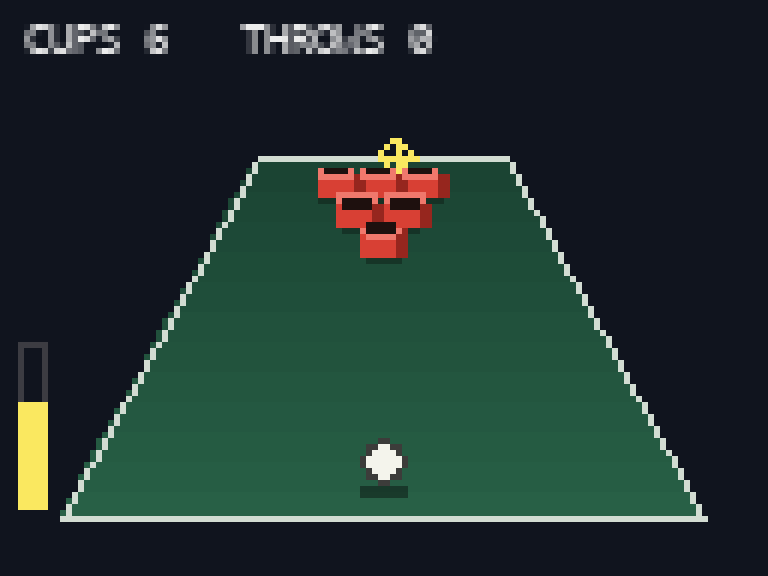
\includegraphics[height=3.0cm]{cup_aim.png}\hfill
  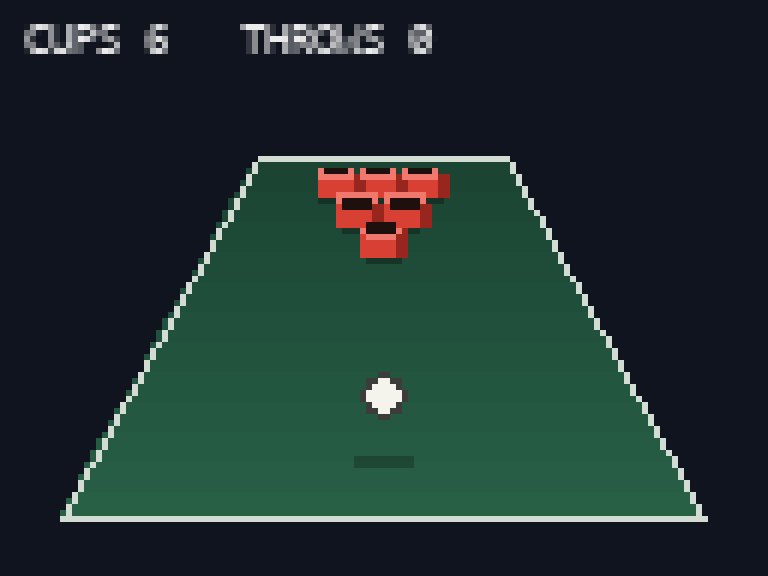
\includegraphics[height=3.0cm]{cup_flight.png}\hfill
  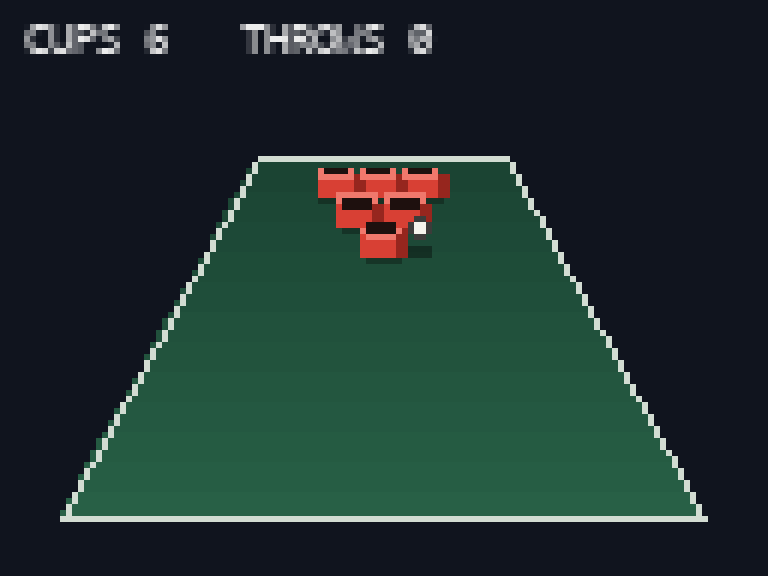
\includegraphics[height=3.0cm]{cup_rimbounce.png}%
}{\fbox{\parbox{0.9\linewidth}{\centering\vspace{2cm}[engine frames: aim / flight / rim-bounce]\vspace{2cm}}}}
\caption{Deterministic engine, $128\times96$ fixed-camera frames: aiming at the rack (left), a ball in flight (center), and a rim-bounce on a graze that does not drop cleanly (right).}
\label{fig:phases}
\end{figure}

\subsection{State, action, and event spaces}

The world state is a $21$-dimensional vector (Table~\ref{tab:state}); the controller action is a $5$-dimensional multi-hot; and the engine emits a $7$-dimensional event vector per step used as an auxiliary training signal.

\begin{table}[h!]
\centering
\caption{The $21$-dimensional structured game state $\stt$. The learned model predicts all of it.}
\label{tab:state}
\begin{tabularx}{\linewidth}{>{\raggedright\arraybackslash}p{0.26\linewidth} c X}
\toprule
Field & Dim & Meaning \\
\midrule
\code{ball\_position} & 3 & ball center $(x,y,z)$ in table-space \\
\code{ball\_velocity} & 3 & ball velocity \\
\code{aim\_x} & 1 & lateral aim, $[-1,1]$ \\
\code{power} & 1 & charge, $[0,1]$ \\
\code{cups\_present} & 6 & per-cup bitmask, $1$ present / $0$ sunk (monotone) \\
\code{score} & 1 & cups sunk $=\!6-\sum\code{cups\_present}$ \\
\code{throws\_used} & 1 & monotone throw counter \\
\code{phase\_onehot} & 4 & AIM / FLIGHT / RESULT / GAME\_OVER \\
\code{result\_timer} & 1 & frozen frames left after a throw lands \\
\bottomrule
\end{tabularx}
\end{table}

Actions are \code{[aim\_left, aim\_right, power\_up, power\_down, throw]}; events are \code{[throw\_released, cup\_sunk, miss, table\_bounce, rim\_bounce, rack\_cleared, game\_over]}. Observations are decoupled from simulation: physics integrates at $60$\,Hz but the agent observes every third step ($20$\,Hz), so a single learned step must summarize three physics ticks.

\subsection{Physics}

At release, the launch speed and direction are set from the trimmed controls,
\begin{equation}
    v_0 = \text{POWER\_MIN} + \code{power}\,(\text{POWER\_MAX}-\text{POWER\_MIN}), \qquad
    \theta = \code{aim\_x}\cdot\text{MAX\_AIM\_ANGLE},\quad \varphi = \text{LAUNCH\_ELEV},
\end{equation}
giving an initial velocity $\vect{v} = v_0\,(\cos\varphi\sin\theta,\ \cos\varphi\cos\theta,\ \sin\varphi)$ from a fixed throw origin, with $\varphi$ held constant so the throw is a one-parameter-per-axis family the player learns to feel. The ball then integrates under gravity,
\begin{equation}
    \vect{v}\leftarrow \vect{v}-g\,\hat{\vect{z}}\,\Delta t,\qquad \vect{p}\leftarrow \vect{p}+\vect{v}\,\Delta t,\qquad g=200,\ \Delta t = 1/60.
\end{equation}

Cup interaction is resolved \emph{only} at the descending crossing of the rim plane $z=\text{CUP\_RIM\_Z}$, which is the honest geometric definition of ``over the cup on the way down.'' Let $c^\star$ be the nearest present cup center to the ball's $(x,y)$ at that crossing, and $d$ the distance to it:
\begin{equation}
    \text{outcome} =
    \begin{cases}
        \textbf{make} & d \le \text{SINK\_RADIUS}=3.3, \\
        \textbf{rim-bounce} & \text{SINK\_RADIUS} < d \le \text{CUP\_R}+\text{BALL\_R}, \\
        \textbf{pass} & \text{otherwise (then test the table for a miss).}
    \end{cases}
\end{equation}
A make removes $c^\star$ from the bitmask and ends the throw; a rim-bounce applies an upward pop and outward horizontal kick (the graze in Figure~\ref{fig:phases}, right); a miss bounces off the table with restitution and ends the throw. The forgiving \code{SINK\_RADIUS} ($<\text{CUP\_R}=4.0$) makes ``visibly over the cup'' drop, which matters greatly once a \emph{learned} ball has to hit it.

\section{Data Generation}

Trajectories are generated by a deterministic scripted thrower. It caches a $(\code{aim\_x},\code{power})\!\to\!\text{landing}$ table by simulating the engine's ballistics on a $41\times41$ grid, selects the grid cell whose true landing is nearest a chosen present cup, and drives the aim/power controls toward it with a skill-scaled jitter so the dataset contains a realistic mix of makes, rims, and misses. Each episode records the full $(\stt_t,\act_t,\text{events}_t)$ stream and, optionally, rendered frames for the visual stage. Because the thrower is seeded, the entire dataset is reproducible from an integer.

\section{Structured Dynamics Model}

\subsection{Architecture}

The dynamics model is a gated recurrent network \cite{gru} with a per-field decoder head (Figure~\ref{fig:dyn}):
\begin{equation}
    \vect{x}_t = \mathrm{enc}([\stt_t,\act_t]),\qquad \vect{h}_t = \mathrm{GRU}(\vect{x}_t,\vect{h}_{t-1}),
\end{equation}
and from $\vect{h}_t$ four heads predict the next state: a continuous head ($11$ dims: position, velocity, aim, power, score, throws, timer), a cups head ($6$ logits), a phase head ($4$ logits), and an auxiliary event head ($7$ logits). The full model is $408{,}860$ parameters.

A key modeling choice is \emph{what} each continuous field predicts. Slowly-drifting quantities (position, aim, power, the counters) are predicted as \textbf{deltas} added to the current value, which keeps the network near identity and stabilizes long rollouts; \textbf{velocity is predicted absolutely} (``direct''), because during flight it changes by a large, near-constant gravitational increment each step that is easier to name outright than to correct incrementally. A normalizer applies per-field $z$-scoring (delta statistics for the delta fields, absolute statistics for velocity) so all heads train on comparable scales.

\subsection{The snap projection}

A raw regression head will happily predict a cup that un-sinks, a fractional throw counter, or an illegal AIM$\to$GAME\_OVER jump. We forbid this with a hard projection operator $\Pi$ (\code{snap}) applied to every predicted next-state, identically in training feedback and at inference (a single source of truth):
\begin{equation}
    \hat{\stt}_{t+1} = \Pi\big(\stt_t,\ \text{heads}(\vect{h}_t)\big).
\end{equation}
$\Pi$ enforces: (i) a legal phase transition, masking the phase logits by an automaton adjacency matrix before the argmax; (ii) \emph{monotone} cups (a present cup may sink but a sunk cup never returns); (iii) $\code{score}=6-\sum\code{cups}$ derived, not predicted; (iv) a rounded, monotone throw counter; (v) bounded aim/power/$z$/timer; and (vi) phase-conditioned \emph{parking}: outside FLIGHT the ball is snapped to the throw origin with zero velocity, so the model never has to ``hold'' a still ball. Snap turns a noisy real-valued prediction into a guaranteed-legal game state, which is what makes engine-off rollouts stay coherent for hundreds of steps.

\begin{figure}[h!]
\centering
\IfFileExists{../assets/neural_t2.png}{%
  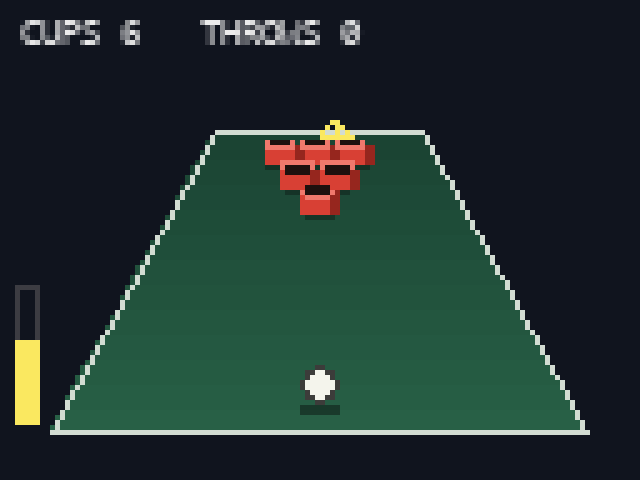
\includegraphics[height=2.7cm]{neural_t2.png}\hfill
  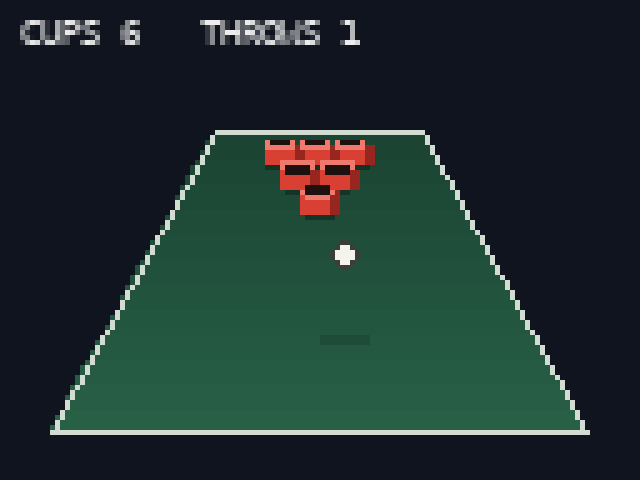
\includegraphics[height=2.7cm]{neural_t20.png}\hfill
  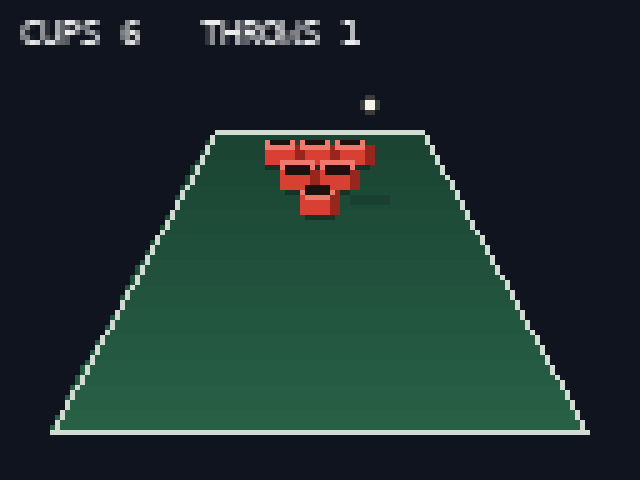
\includegraphics[height=2.7cm]{neural_t30.png}%
}{\fbox{\parbox{0.9\linewidth}{\centering\vspace{1.8cm}[engine-off rollout frames $t=2,20,30$]\vspace{1.8cm}}}}
\caption{Engine \emph{off}: the GRU alone advances the structured state, drawn here by the real renderer (Mode F2), at steps $t=2,20,30$ of a free-run rollout under player actions.}
\label{fig:dyn}
\end{figure}

\section{Training Curriculum and Losses}

\subsection{Curriculum}

Training uses a two-phase curriculum. \textbf{Teacher forcing} first fits local dynamics: the model sees ground-truth states and predicts one step ahead, which converges fast and nails aim/power/phase. \textbf{Scheduled sampling} \cite{scheduledsampling} then fights exposure bias: the model is fed its own \code{snap}-projected predictions with probability $1-p$, annealed over training, so it learns to recover from its own small errors instead of only ever seeing clean inputs. We warm the hidden state on a short ground-truth burn-in, then free-run a horizon of $24$ steps. A gentle schedule (final teacher-forcing probability $0.4$) was necessary: more aggressive free-running destabilized the ballistic parts of the rollout. We keep the checkpoint with the best free-run positional rollout proxy on a fixed validation batch rather than the last epoch.

\subsection{Loss}

The per-field loss is a weighted Huber in normalized space for the continuous head, BCE for cups and events, and cross-entropy for phase, with two masks that steer gradient toward the hard ticks:
\begin{equation}
    \mathcal{L} = \underbrace{\big\| w \odot \mathrm{Huber}(\hat{c},c)\big\|}_{\text{continuous}}
    + \lambda_{\text{cups}}\,\mathcal{L}_{\text{cups}}
    + \lambda_{\text{phase}}\,\mathcal{L}_{\text{phase}}
    + \lambda_{\text{event}}\,\mathcal{L}_{\text{event}}.
\end{equation}
A \emph{motion} mask upweights moving/flight frames (where position error compounds along the arc) and a \emph{transition} mask upweights the sparse throw/sink/land ticks. Because a cup-sink is a rare one-tick $1\!\to\!0$ flip in the bitmask, the cups BCE additionally upweights flip frames heavily and we oversample sink windows in the batch sampler, both aimed at stopping the cups head from collapsing to ``never change.'' (As Section~\ref{sec:wall} shows, these help the head fire but cannot by themselves make the game sink, because the problem lies upstream in the predicted ball.)

\section{Neural Rendering: The State-Grounded Latent Renderer}

The visual stage learns $\stt\mapsto$ frame so the game can be drawn without the engine's renderer. A conv decoder asked to invent a $128\times96$ scene from a $21$-vector produces blotchy felt and garbled HUD text. The fix is to \emph{ground} the decoder in geometry it should not have to hallucinate.

We rasterize the state into a stack of $16$ hint channels using the PyTorch port of the camera projection: Gaussian blobs for the ball and its shadow, filled disks for each \emph{present} cup (gated by the bitmask), the aim reticle and power bar, a phase one-hot broadcast, and, crucially, three channels of a \emph{static empty-court backdrop}. The decoder is a small upsampling conv net ($261{,}891$ parameters) with FiLM conditioning \cite{film} from the state vector, trained with a \emph{foreground-weighted} $L_1$ loss that pays more for the ball, cups, and HUD than for the static felt. Adding the backdrop hint channels alone cut held-out reconstruction from $L_1=0.048$ to $\mathbf{0.0077}$. Figure~\ref{fig:decoder} shows ground-truth versus decoder output.

\begin{figure}[h!]
\centering
\IfFileExists{../assets/phase5_gt_vs_neural.png}{%
  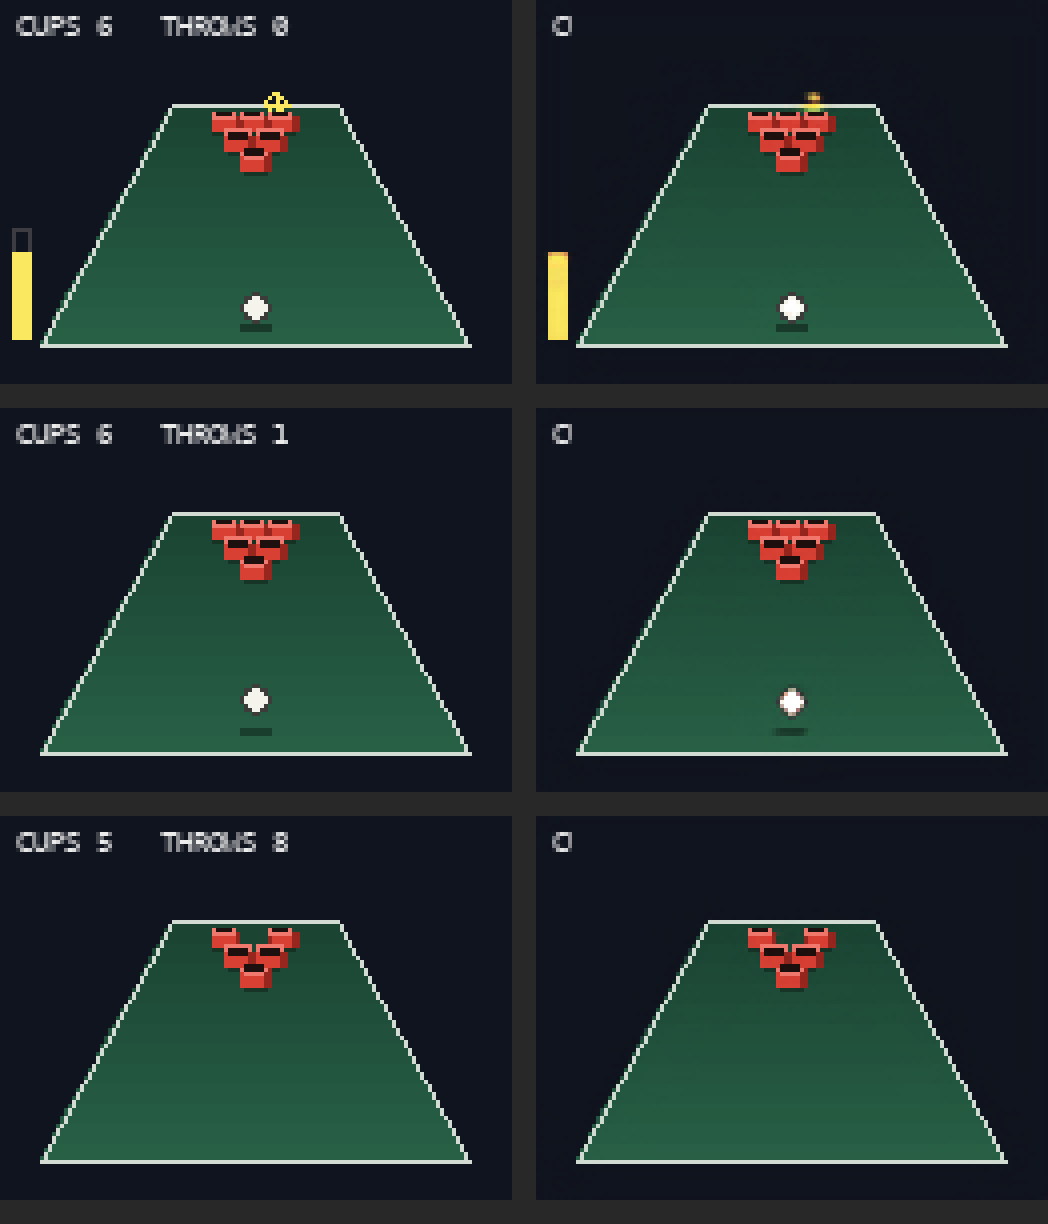
\includegraphics[width=0.86\linewidth]{phase5_gt_vs_neural.png}%
}{\fbox{\parbox{0.9\linewidth}{\centering\vspace{2.2cm}[ground-truth vs.\ neural-decoder frames]\vspace{2.2cm}}}}
\caption{State-grounded latent renderer. Top: engine-rendered ground truth. Bottom: the $262$K-parameter decoder's output from the same states (engine renderer \emph{off}). Held-out $L_1 = 0.0077$.}
\label{fig:decoder}
\end{figure}

\section{Inference Modes}

The playable build exposes three modes that switch off progressively more of the hand-written stack:

\begin{table}[h!]
\centering
\caption{What is real and what is neural in each play mode.}
\label{tab:modes}
\begin{tabularx}{\linewidth}{>{\bfseries}p{0.06\linewidth} X X X}
\toprule
Mode & World dynamics & Rendering & Role \\
\midrule
F1 & deterministic engine & engine renderer & ground-truth reference \\
F2 & \textbf{GRU} (engine off) & engine renderer & pure learned-dynamics demo \\
F3 & \textbf{hybrid} (engine off) & \textbf{neural decoder} (renderer off) & fully-generated, playable \\
\bottomrule
\end{tabularx}
\end{table}

In F2 the network alone advances the structured state under live controller input (Figure~\ref{fig:dyn}); in F3 both the engine and its renderer are off and the game you see and play is produced entirely by the two networks (Figure~\ref{fig:f3}). The controls, HUD, and win condition are identical across modes.

\section{Results}

\subsection{Control and short-horizon dynamics}

On held-out seeds the learned dynamics is excellent at everything except ballistic landing (Table~\ref{tab:results}). One-step aim and power errors are $0.0025$ and $0.0013$ on their $[-1,1]$/$[0,1]$ scales; phase transitions are $99.4\%$ correct; the throw counter is exact; and controllability (does the world move the way the button says?) is a perfect $100\%$ directional-response rate for aim, power, and throw-launch. Subjectively this is what makes F2/F3 feel like the game rather than like a video of it.

\begin{table}[h!]
\centering
\caption{Learned-model evaluation (held-out seeds). Position error in table-units; aim/power on normalized control scales.}
\label{tab:results}
\begin{tabularx}{\linewidth}{X r}
\toprule
Metric & Value \\
\midrule
Dynamics GRU parameters & $408{,}860$ \\
Neural decoder parameters & $261{,}891$ \\
\midrule
One-step position RMSE & $0.887$\,u \\
One-step aim / power MAE & $0.0025$ / $0.0013$ \\
One-step cups / phase accuracy & $0.998$ / $0.994$ \\
One-step throw-count exactness & $1.000$ \\
Controllability (aim / power / throw dir-rate) & $1.00$ / $1.00$ / $1.00$ \\
\midrule
Rollout position RMSE @ $H{=}5$ / $10$ / $30$ & $5.2$ / $8.3$ / $22.4$\,u \\
Median steps until divergence & $14$ \\
Legal-state (invariant) rate over rollout & $1.00$ \\
Whole-game score MAE vs.\ engine & $2.8$ \\
\midrule
Decoder held-out $L_1$ (with backdrop hints) & $0.0077$ \\
Camera-projection port error vs.\ engine & $0.0$\,px \\
\bottomrule
\end{tabularx}
\end{table}

\subsection{Long-horizon drift}

Free-run rollouts stay \emph{legal} indefinitely (snap guarantees it: invariant rate $1.00$) but drift in continuous value: positional RMSE grows to $\approx 22$u by $30$ steps, and the median trajectory measurably diverges from the engine's after $\sim 14$ steps. The whole-game score MAE against the engine is $\approx 2.8$ cups. The dominant contributor to that drift is exactly the flight phase, which motivates the next section.

\section{The Flight-Precision Wall}
\label{sec:wall}

\subsection{Symptom}

Played in F2/F3, the game felt right until you tried to \emph{score}: the ball would arc plausibly, the felt and cups and HUD all rendered cleanly, but cups almost never sank. Instrumenting the make-rate confirmed it: the fully-learned mode sank roughly $3\%$ of well-aimed throws, against the engine's $100\%$.

\subsection{Diagnosis}

We first blamed the sink resolution and attacked it three ways: (i) upweighting the rare cup-flip in the BCE by $25\times$; (ii) oversampling sink windows in the batch sampler; and (iii) adding a \emph{rule-based sink} to the snap operator that drops a cup whenever the model's \emph{predicted} descending ball passes within \code{SINK\_RADIUS} of a present cup. None moved the make-rate. Tracing an individual throw explained why:

\keybox{\textbf{Root cause.} With the bot aiming dead-on a cup at $(30,90)$, the \emph{engine's} ball passes $0.31$\,u from the cup center at the rim plane, a clean make. The \emph{GRU's predicted} ball, given the same intent, never gets closer than $\mathbf{8.4}$\,\textbf{u}. The predicted arc looks reasonable ($z$ rises to $\sim37$ and falls) but its \emph{landing} is off by more than a cup diameter. The ball simply is not at the cup, so no sink head, loss weight, or snap rule can drop it.}

This is a capacity limit, not a bug. Localizing a $60$-Hz ballistic landing over an $\sim 85$-unit throw to within a $3.3$-unit radius demands that a $409$K recurrent model integrate a fast arc almost exactly, and small errors in the predicted launch velocity, compounded over the flight, land well outside the cup. The same model that tracks aim to $0.0025$ cannot pin the landing, because landing precision is a far harder function of the launch than direction-following is. More training did not close the gap; more capacity might, but that abandons the ``how small can it be'' premise.

\subsection{Fix: the hybrid world model}

The resolution keeps the network where it is strong and defers to physics where it is weak. At release, the ball's velocity is seeded from the network's \emph{own} aim and power (which it tracks to $\approx 0.002$, so the seed is accurate) and the arc is then integrated with the exact, deterministic ballistics and sink test, while the GRU continues to drive aim, power, and the phase machine, and the decoder continues to render:
\begin{equation}
    \underbrace{\text{aim, power, phase}}_{\text{neural (GRU)}}\ \longrightarrow\
    \underbrace{\text{ballistic arc + sink/miss}}_{\text{exact physics, seeded from neural control}}\ \longrightarrow\
    \underbrace{\text{pixels}}_{\text{neural (decoder)}} .
\end{equation}
This is the ``hybrid flight'' mode (F3). It sinks $\mathbf{6/6}$ cups, matching the engine exactly, and a regression test locks in engine-parity sinking for every cup in the rack. The pure-learned F2 mode is retained as the honest artifact: it shows what the structured dynamics does and does not learn, flight wall included.

\begin{figure}[h!]
\centering
\IfFileExists{../assets/f3_sink.png}{%
  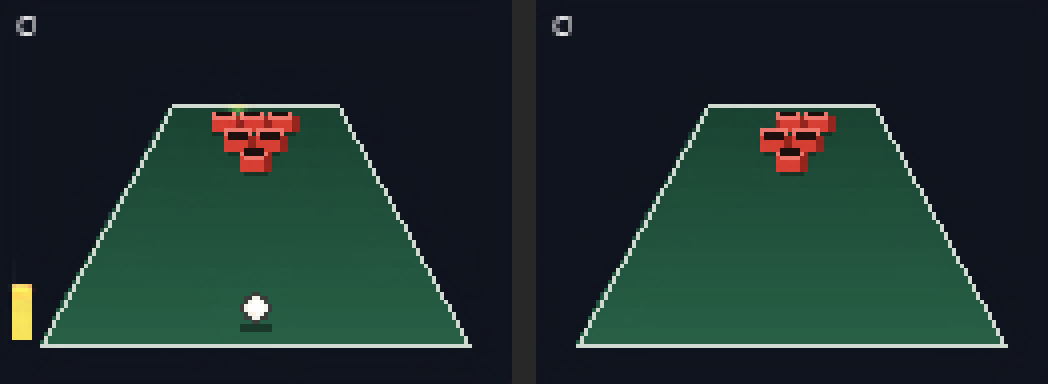
\includegraphics[height=3.0cm]{f3_sink.png}\hfill
  \IfFileExists{../assets/phase6_fully_generated.png}{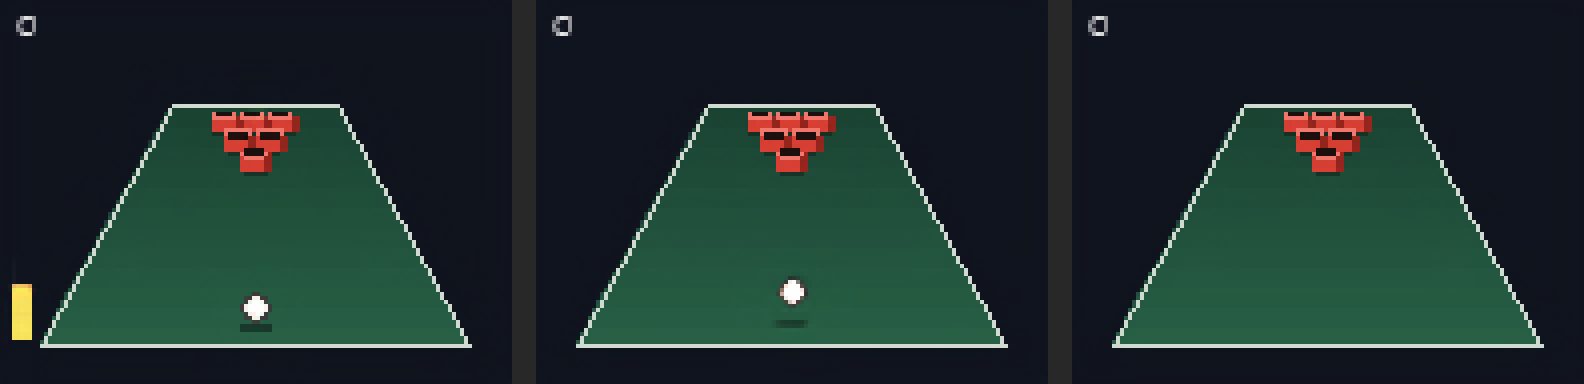
\includegraphics[height=3.0cm]{phase6_fully_generated.png}}{}%
}{\fbox{\parbox{0.9\linewidth}{\centering\vspace{2cm}[F3 hybrid: a cup sinking, fully generated]\vspace{2cm}}}}
\caption{Mode F3 (engine \emph{and} renderer off): the hybrid world model sinks a cup, with every pixel produced by the neural decoder. Neural control $+$ exact flight $+$ neural rendering.}
\label{fig:f3}
\end{figure}

\subsection{What the hybrid concedes, and why it is the right call}

Honesty demands stating the concession: in F3 the ball's \emph{arc} is real physics, not learned. Everything else is neural: the interactive control loop, the phase/score logic driven off the network's predictions, and $100\%$ of the pixels. The trade buys engine-parity playability for the one faculty a small structured model provably cannot supply. For a game whose entire point is to \emph{sink cups}, that is the correct place to spend a rule. The alternative, a pure-learned mode that arcs beautifully and never scores, is a better research curiosity and a worse game, and both are shipped so the reader can feel the difference.

\section{Discussion, Limitations, and Future Work}

\begin{itemize}
    \item \textbf{The wall is the finding.} The interesting result is not that a tiny world model works; it is precisely \emph{where} it stops working. Control-following and discrete state logic are cheap to learn; sub-cup ballistic localization is not. A world model's weakest link is whichever variable is a sensitive, compounding function of an early continuous choice.
    \item \textbf{Could a pure model clear the wall?} Plausibly, via a launch-velocity representation that predicts the whole arc from the release conditions in closed form rather than integrating it step-by-step, or simply more capacity. Both are worth trying but neither is ``small.''
    \item \textbf{Rendering is the easy, satisfying part.} The state-grounded decoder is the component that most feels like magic and was the least troublesome, because geometry hints do the heavy lifting; the network only has to shade and antialias. Removing hint channels one at a time would quantify how much it has actually learned to synthesize.
    \item \textbf{Drift.} Even with legal-state guarantees, continuous drift over long rollouts remains; a learned correction term or periodic re-grounding could extend coherent horizons.
    \item \textbf{Scope.} This is a hobby project on an original game; all art and physics are hand-made. Nothing here targets or reproduces a commercial title.
\end{itemize}

\section{Conclusion}

Neural Cup Pong is a fully playable arcade game in which, at the strongest setting, no game engine and no graphics renderer run: a $409$K-parameter recurrent dynamics model driven by a legality-preserving projection handles control and state, and a $262$K-parameter state-grounded decoder paints every frame. The build is honest about its one hard limit, that a small structured model cannot localize a ballistic landing to within a cup, and resolves it with a hybrid that seeds exact flight from the network's own accurate control, restoring engine-parity sinking while keeping control and rendering neural. The lesson generalizes past cup pong: when you shrink a world model, the first thing to break is the variable that is a sensitive, compounding function of a continuous action, and the pragmatic fix is to learn everything else and hand that one variable back to physics.

\newpage
\begin{thebibliography}{99}

\bibitem{worldmodels}
David Ha and J\"urgen Schmidhuber.
\newblock \textit{World Models}.
\newblock 2018.
\newblock \url{https://arxiv.org/abs/1803.10122}

\bibitem{dreamerv3}
Danijar Hafner, Jurgis Pasukonis, Jimmy Ba, and Timothy Lillicrap.
\newblock \textit{Mastering Diverse Domains through World Models (DreamerV3)}.
\newblock 2023.
\newblock \url{https://arxiv.org/abs/2301.04104}

\bibitem{diamond}
Eloi Alonso, Adam Jelley, Vincent Micheli, Anssi Kanervisto, Amos Storkey, Tim Pearce, and Fran\c{c}ois Fleuret.
\newblock \textit{Diffusion for World Modeling: Visual Details Matter in Atari (DIAMOND)}.
\newblock NeurIPS, 2024.
\newblock \url{https://arxiv.org/abs/2405.12399}

\bibitem{gamengen}
Dani Valevski, Yaniv Leviathan, Moab Arar, and Shlomi Fruchter.
\newblock \textit{Diffusion Models Are Real-Time Game Engines (GameNGen)}.
\newblock 2024.
\newblock \url{https://arxiv.org/abs/2408.14837}

\bibitem{genie}
Jake Bruce, Michael Dennis, Ashley Edwards, Jack Parker-Holder, et al.
\newblock \textit{Genie: Generative Interactive Environments}.
\newblock ICML, 2024.
\newblock \url{https://arxiv.org/abs/2402.15391}

\bibitem{gru}
Kyunghyun Cho, Bart van Merri\"enboer, Caglar Gulcehre, Dzmitry Bahdanau, Fethi Bougares, Holger Schwenk, and Yoshua Bengio.
\newblock \textit{Learning Phrase Representations using RNN Encoder--Decoder for Statistical Machine Translation}.
\newblock EMNLP, 2014.
\newblock \url{https://arxiv.org/abs/1406.1078}

\bibitem{scheduledsampling}
Samy Bengio, Oriol Vinyals, Navdeep Jaitly, and Noam Shazeer.
\newblock \textit{Scheduled Sampling for Sequence Prediction with Recurrent Neural Networks}.
\newblock NeurIPS, 2015.
\newblock \url{https://arxiv.org/abs/1506.03099}

\bibitem{film}
Ethan Perez, Florian Strub, Harm de Vries, Vincent Dumoulin, and Aaron Courville.
\newblock \textit{FiLM: Visual Reasoning with a General Conditioning Layer}.
\newblock AAAI, 2018.
\newblock \url{https://arxiv.org/abs/1709.07871}

\bibitem{diffusion_policy}
Cheng Chi, Zhenjia Xu, Siyuan Feng, Eric Cousineau, Yilun Du, Benjamin Burchfiel, Russ Tedrake, and Shuran Song.
\newblock \textit{Diffusion Policy: Visuomotor Policy Learning via Action Diffusion}.
\newblock RSS, 2023.
\newblock \url{https://arxiv.org/abs/2303.04137}

\end{thebibliography}

\end{document}
